\documentclass[g5paper,10pt,final,openright,coverpage,swedish]{thesis}

%% Standard packages
\usepackage{xcolor}
\usepackage{graphicx}
\usepackage{amsmath}
\usepackage{pdfpages}
\usepackage[hidelinks]{hyperref}

%% Epigraphs
\usepackage{epigraph}

%% Bibliography
\usepackage[citestyle=authoryear,
bibstyle=authoryear,
sorting=nyt,
backend=bibtex,
natbib]{biblatex}
\setlength\bibitemsep{0.5\baselineskip}
%\addbibresource{Thesis_bibliography.bib}

%% Document information 
\title{Thesis title}
\author{Your Name}
\date{May 2020}
\shortdate{2020}
\type{Doctoral Thesis in Physics}
\division{Particle and Astroparticle Physics}
\department{Department of Physics}
\address{SE-106 91 Stockholm, Sweden}
\city{Stockholm}
\country{Sweden}
\publisher{Printed by Universitetsservice US-AB}
\copyrightline{\copyright\ Your Name, May 2020}
\trita{Get from administration/online}
\isbn{Get from administration/online}

%\issn{}
%\isrn{}
%\isrn{KTH/FYS/\mbox{-}\mbox{-}16:81\mbox{-}\mbox{-}SE}
%TRITA-FYS 2016:81
%ISSN 0280-316X
%ISRN KTH/FYS/--16:81—SE

\cplogo{kth_svv.png}
\cplogonblines{1} % Number of text lines below kth logo... don't ask..
%\cpillustration{image_filename} % Front page image
\innerlogo{
\includegraphics[width=32mm]{kth_svv.png}}
\centercomment{Cover illustration: } 
\foregincomment{Akademisk avhandling som med tillst{\aa}nd av Kungliga Tekniska h{\"o}gskolan i Stockholm framl{\"a}gges till offentlig granskning f{\"o}r avl{\"a}ggande av teknologie doktorsexamen [date, time, and place], AlbaNova Universitetscentrum, Roslagstullsbacken 21, Stockholm.\\ \\ Avhandlingen f{\"o}rsvaras p{\aa} engelska.}

%% Command for small comments in the margin
\newcommand{\n}[1]{\marginpar[\raggedleft\scriptsize\textsf{#1}]{\raggedright\scriptsize\textsf{#1}}}
\newcommand{\beq}{\begin{equation}}
\newcommand{\eeq}{\end{equation}}

%% Journal abbreviations
\newcommand\aap{{A\&A}}      
\newcommand\apj{{ApJ}}       
\newcommand\apjs{{ApJS}}     
\newcommand\apjl{{ApJL}}     
\newcommand\mnras{{MNRAS}}   
\newcommand\physrep{{Physics Reports}} 
\newcommand\nat{{Nature}}    
\newcommand{\apss}{Ap\&SS}

%% Useful commands
\newcommand{\todo}[1]{(\textbf{TODO:} #1)}
\newcommand{\ud}{\mathrm{d}}
\newcommand{\dd}[2]{\frac{{\rm d}#1}{{\rm d}#2}}
\newcommand{\Fig}{[{\bf FIG}]}
\newcommand{\chk}{[{\bf CHECK}]}


%% Style hacks
%\makeatletter
%\g@addto@macro\@floatboxreset\centering
%\newcommand*{\rom}[1]{\expandafter\@slowromancap\romannumeral #1@}
%\makeatother


%% MAIN DOCUMENT %%

\begin{document}

\maketitle

\cleardoublepage

%% Abstract

\chapter{Abstract}
\label{ch:abstract}

\lipsum[1]
\addcontentsline{toc}{chapter}{Abstract}

%% Sammanfattning

\chapter{Sammanfattning}
\label{ch:sammanfattning}

\lipsum[1]

\addcontentsline{toc}{chapter}{Sammanfattning}

\tableofcontents

%% Introduction
%% Introduction

\chapter{Introduction}
\label{ch:intro}

\lipsum[10-20]

%% Paper summary 
%% Paper summary

\chapter{\label{ch:paper_summary}Publication list}

\begin{zeroindent}

  \section*{Publications included in the thesis}
  
  \subsection*{Paper~I}

  \textbf{Name, A.} et al., 2020, Article title. \textit{Journal}, 10, 99.

  \href{https://doi.org/}{\texttt{DOI}}

  \href{https://arxiv.org/}{\texttt{arXiv:identifier}}

  \subsection*{Paper~II}  


  \subsection*{Paper~III}

  
  
  \section*{Additional publications not included in the thesis}

  \subsection*{Paper~4}


  \subsection*{Paper~5}


  \subsection*{Paper~6}
  
  
\end{zeroindent}

\addcontentsline{toc}{chapter}{Summary of the attached papers}

%% Author contribution
\include{Author_contribution}
\addcontentsline{toc}{chapter}{Author's contribution to the attached papers}

%% Acknowledgements
\include{acknowledgments}
\addcontentsline{toc}{chapter}{Acknowledgements}

% This separates the introduction from the main part of the thesis.
\mainmatter

%% Chapters
\cleardoublepage
%%% Chapter one

\chapter{Chapter one}
\label{ch:one}

\newacronym{yolo}{YOLO}{You only live once}

\lipsum[30-40]

\begin{figure}
  \centering
  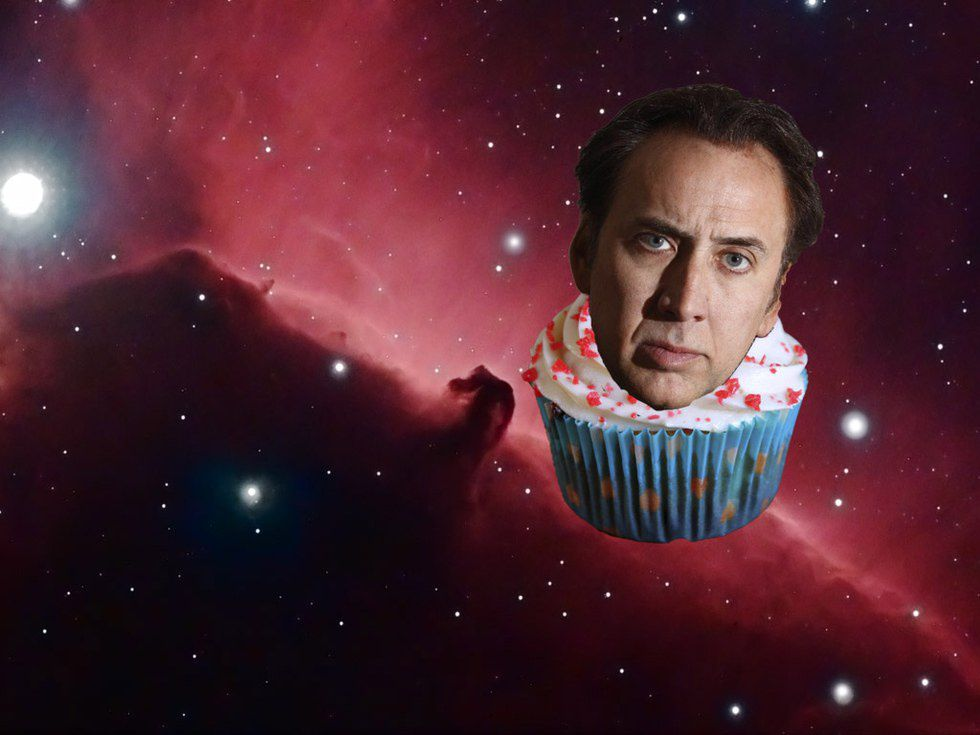
\includegraphics[width=0.4\textwidth]{figures/cupcake1.jpg}
  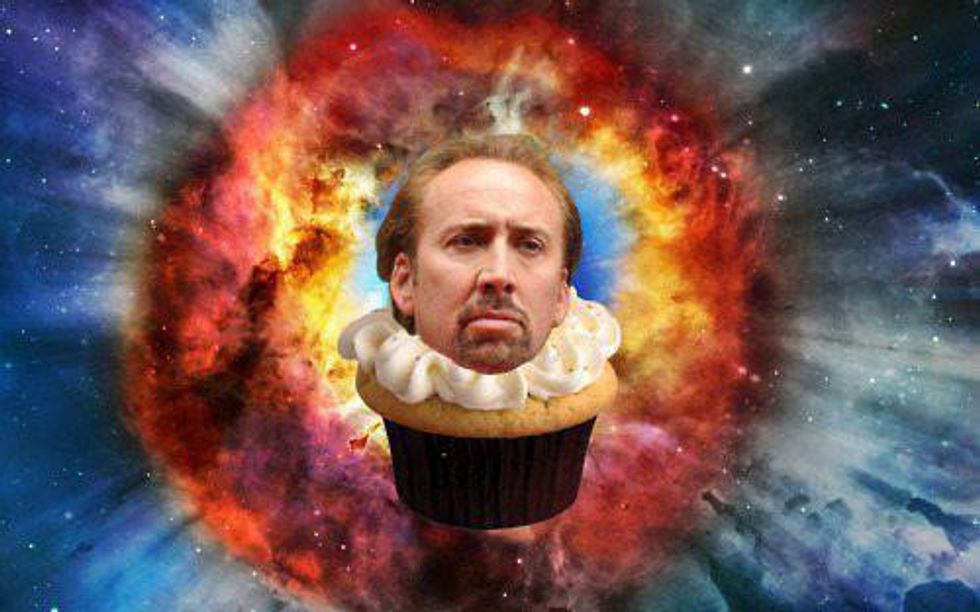
\includegraphics[width=0.4\textwidth]{figures/cupcake2.jpg}
  \caption{Nicolas Cage as a cupcake in space. Figures taken from \citet{reference}.}
  \label{fig:nic_cake}
\end{figure}

\lipsum[41-3]

%%% Chapter one

\chapter{Chapter two}
\label{ch:one}

\lipsum[41-50]

 \begin{table}[ht]
\centering
\begin{tabular}{cc}
  \toprule
  \multicolumn{2}{c}{A simple table} \\ \midrule
  1 & 2 \\
  3 & 4 \\
  \bottomrule
\end{tabular}
\caption{A table.} 
\end{table}

\lipsum[51]

%% List of tables 
%\addcontentsline{toc}{chapter}{List of tables}
%\listoftables

%% List of figures 
\addcontentsline{toc}{chapter}{List of figures}
\listoffigures

%% Bibliography 
\cleardoublepage
\addcontentsline{toc}{chapter}{Bibliography}

\printbibliography
\cleardoublepage

%% Papers
\addcontentsline{toc}{chapter}{Papers}
\part*{Scientific papers}
%\label{papers}
%\includepdf[pages={1-5}]{}
%\includepdf[pages={1-}]{}
%\includepdf[pages={1-}]{}

\end{document}
